% Options for packages loaded elsewhere
\PassOptionsToPackage{unicode}{hyperref}
\PassOptionsToPackage{hyphens}{url}
%
\documentclass[
]{article}
\usepackage{amsmath,amssymb}
\usepackage{iftex}
\ifPDFTeX
  \usepackage[T1]{fontenc}
  \usepackage[utf8]{inputenc}
  \usepackage{textcomp} % provide euro and other symbols
\else % if luatex or xetex
  \usepackage{unicode-math} % this also loads fontspec
  \defaultfontfeatures{Scale=MatchLowercase}
  \defaultfontfeatures[\rmfamily]{Ligatures=TeX,Scale=1}
\fi
\usepackage{lmodern}
\ifPDFTeX\else
  % xetex/luatex font selection
\fi
% Use upquote if available, for straight quotes in verbatim environments
\IfFileExists{upquote.sty}{\usepackage{upquote}}{}
\IfFileExists{microtype.sty}{% use microtype if available
  \usepackage[]{microtype}
  \UseMicrotypeSet[protrusion]{basicmath} % disable protrusion for tt fonts
}{}
\makeatletter
\@ifundefined{KOMAClassName}{% if non-KOMA class
  \IfFileExists{parskip.sty}{%
    \usepackage{parskip}
  }{% else
    \setlength{\parindent}{0pt}
    \setlength{\parskip}{6pt plus 2pt minus 1pt}}
}{% if KOMA class
  \KOMAoptions{parskip=half}}
\makeatother
\usepackage{xcolor}
\usepackage[margin=1in]{geometry}
\usepackage{color}
\usepackage{fancyvrb}
\newcommand{\VerbBar}{|}
\newcommand{\VERB}{\Verb[commandchars=\\\{\}]}
\DefineVerbatimEnvironment{Highlighting}{Verbatim}{commandchars=\\\{\}}
% Add ',fontsize=\small' for more characters per line
\usepackage{framed}
\definecolor{shadecolor}{RGB}{248,248,248}
\newenvironment{Shaded}{\begin{snugshade}}{\end{snugshade}}
\newcommand{\AlertTok}[1]{\textcolor[rgb]{0.94,0.16,0.16}{#1}}
\newcommand{\AnnotationTok}[1]{\textcolor[rgb]{0.56,0.35,0.01}{\textbf{\textit{#1}}}}
\newcommand{\AttributeTok}[1]{\textcolor[rgb]{0.13,0.29,0.53}{#1}}
\newcommand{\BaseNTok}[1]{\textcolor[rgb]{0.00,0.00,0.81}{#1}}
\newcommand{\BuiltInTok}[1]{#1}
\newcommand{\CharTok}[1]{\textcolor[rgb]{0.31,0.60,0.02}{#1}}
\newcommand{\CommentTok}[1]{\textcolor[rgb]{0.56,0.35,0.01}{\textit{#1}}}
\newcommand{\CommentVarTok}[1]{\textcolor[rgb]{0.56,0.35,0.01}{\textbf{\textit{#1}}}}
\newcommand{\ConstantTok}[1]{\textcolor[rgb]{0.56,0.35,0.01}{#1}}
\newcommand{\ControlFlowTok}[1]{\textcolor[rgb]{0.13,0.29,0.53}{\textbf{#1}}}
\newcommand{\DataTypeTok}[1]{\textcolor[rgb]{0.13,0.29,0.53}{#1}}
\newcommand{\DecValTok}[1]{\textcolor[rgb]{0.00,0.00,0.81}{#1}}
\newcommand{\DocumentationTok}[1]{\textcolor[rgb]{0.56,0.35,0.01}{\textbf{\textit{#1}}}}
\newcommand{\ErrorTok}[1]{\textcolor[rgb]{0.64,0.00,0.00}{\textbf{#1}}}
\newcommand{\ExtensionTok}[1]{#1}
\newcommand{\FloatTok}[1]{\textcolor[rgb]{0.00,0.00,0.81}{#1}}
\newcommand{\FunctionTok}[1]{\textcolor[rgb]{0.13,0.29,0.53}{\textbf{#1}}}
\newcommand{\ImportTok}[1]{#1}
\newcommand{\InformationTok}[1]{\textcolor[rgb]{0.56,0.35,0.01}{\textbf{\textit{#1}}}}
\newcommand{\KeywordTok}[1]{\textcolor[rgb]{0.13,0.29,0.53}{\textbf{#1}}}
\newcommand{\NormalTok}[1]{#1}
\newcommand{\OperatorTok}[1]{\textcolor[rgb]{0.81,0.36,0.00}{\textbf{#1}}}
\newcommand{\OtherTok}[1]{\textcolor[rgb]{0.56,0.35,0.01}{#1}}
\newcommand{\PreprocessorTok}[1]{\textcolor[rgb]{0.56,0.35,0.01}{\textit{#1}}}
\newcommand{\RegionMarkerTok}[1]{#1}
\newcommand{\SpecialCharTok}[1]{\textcolor[rgb]{0.81,0.36,0.00}{\textbf{#1}}}
\newcommand{\SpecialStringTok}[1]{\textcolor[rgb]{0.31,0.60,0.02}{#1}}
\newcommand{\StringTok}[1]{\textcolor[rgb]{0.31,0.60,0.02}{#1}}
\newcommand{\VariableTok}[1]{\textcolor[rgb]{0.00,0.00,0.00}{#1}}
\newcommand{\VerbatimStringTok}[1]{\textcolor[rgb]{0.31,0.60,0.02}{#1}}
\newcommand{\WarningTok}[1]{\textcolor[rgb]{0.56,0.35,0.01}{\textbf{\textit{#1}}}}
\usepackage{graphicx}
\makeatletter
\def\maxwidth{\ifdim\Gin@nat@width>\linewidth\linewidth\else\Gin@nat@width\fi}
\def\maxheight{\ifdim\Gin@nat@height>\textheight\textheight\else\Gin@nat@height\fi}
\makeatother
% Scale images if necessary, so that they will not overflow the page
% margins by default, and it is still possible to overwrite the defaults
% using explicit options in \includegraphics[width, height, ...]{}
\setkeys{Gin}{width=\maxwidth,height=\maxheight,keepaspectratio}
% Set default figure placement to htbp
\makeatletter
\def\fps@figure{htbp}
\makeatother
\setlength{\emergencystretch}{3em} % prevent overfull lines
\providecommand{\tightlist}{%
  \setlength{\itemsep}{0pt}\setlength{\parskip}{0pt}}
\setcounter{secnumdepth}{-\maxdimen} % remove section numbering
\ifLuaTeX
  \usepackage{selnolig}  % disable illegal ligatures
\fi
\IfFileExists{bookmark.sty}{\usepackage{bookmark}}{\usepackage{hyperref}}
\IfFileExists{xurl.sty}{\usepackage{xurl}}{} % add URL line breaks if available
\urlstyle{same}
\hypersetup{
  pdftitle={Integration by Monte Carlo},
  pdfauthor={Alex Shen},
  hidelinks,
  pdfcreator={LaTeX via pandoc}}

\title{Integration by Monte Carlo}
\author{Alex Shen}
\date{2023-11-13}

\begin{document}
\maketitle

{
\setcounter{tocdepth}{2}
\tableofcontents
}
\hypertarget{the-integration-problem}{%
\subsection{The integration problem}\label{the-integration-problem}}

How to solve the integral of (sin(50x)+cos(20x))\^{}2 from 0 to 1
\[\int_0^1 [sin(50x)+cos(20x)]^2 dx\]

There are couple of ways we do it, for instance checking it online web,
integrating it analytically, or using numerical method, or Monte Carlo
method.

First, Let us ask the big boss of chat.GPT. It turns out a disaster:-)
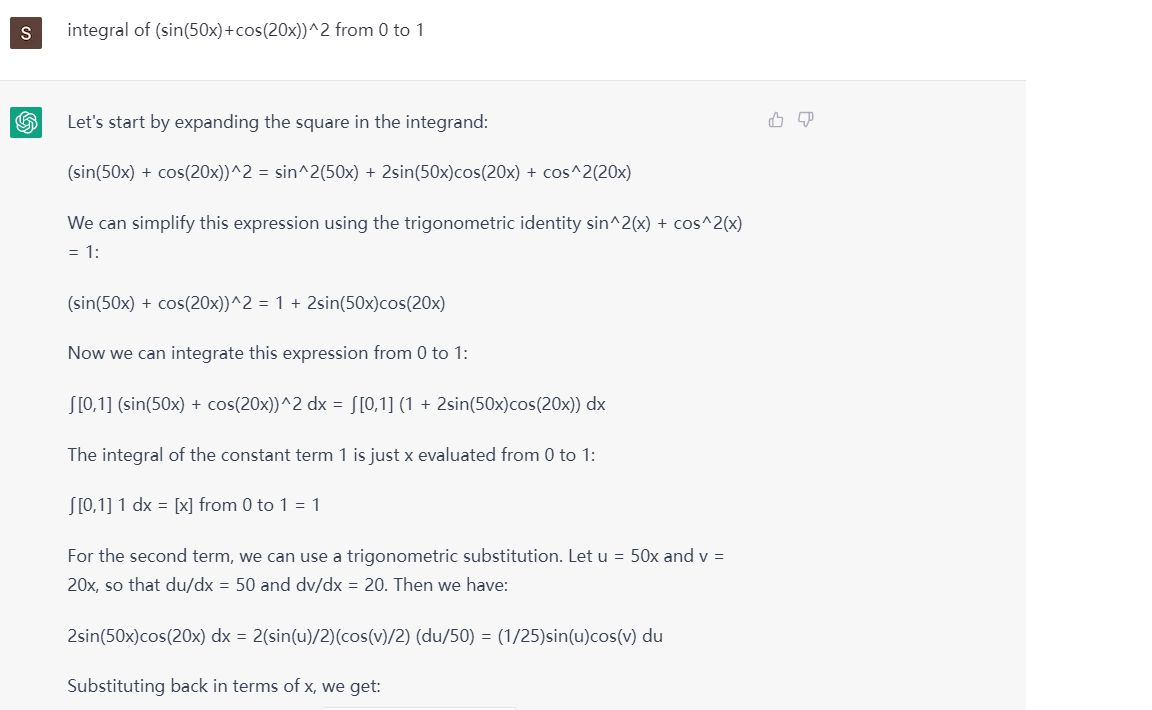
\includegraphics{./fig/chat.gpt.png}

Secondly, Let's try WolframAlpha online

\begin{itemize}
\tightlist
\item
  Copy ``Integral of (sin(50x)+cos(20x))\^{}2 from 0 to 1''
\item
  Paste it into \href{https://www.wolframalpha.com/}{WolframAlpha}
\item
  The engine will translate it into a correct math integral, and give it
  back a number and a very nice visual representation of the integral
  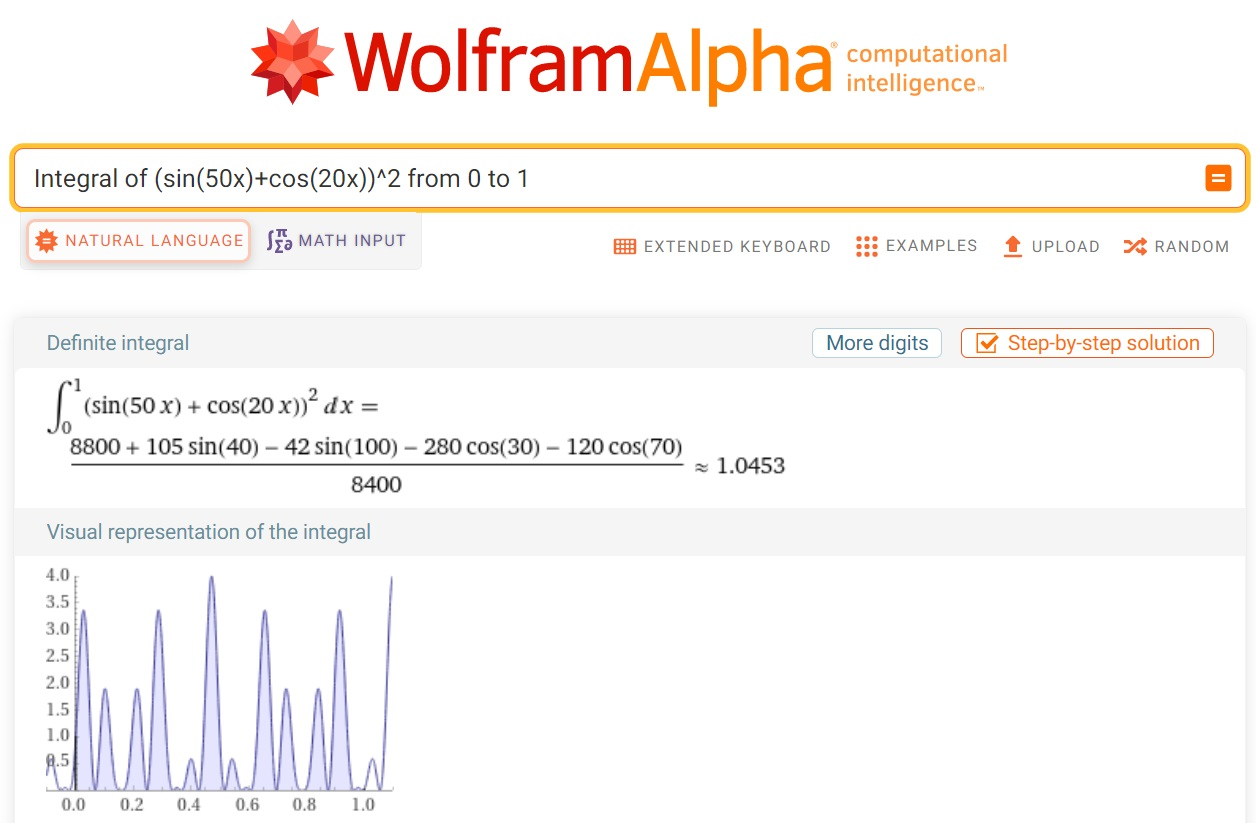
\includegraphics{./fig/math.fig.jpg}
\end{itemize}

\hypertarget{analytic-method}{%
\subsection{Analytic method}\label{analytic-method}}

This is the preferable method, but many integrals may be hard or even
impossible.

\begin{align*}
I  & = \int_0^1 [sin(50x)+cos(20x)]^2 \, dx\\
& =\int_0^1 [sin^2(50x)+cos^2(20x)+2sin(50x)cos(20x)]\, dx\\
& =\int_0^1 [\frac{1-cos(100x)}{2}+\frac{1+cos(40x)}{2}+sin(50x+20x)+sin(50x-20x)]\, dx\\
& =\left[\frac{1}{2}x-\frac{1}{2}\frac{sin(100x)}{100}+\frac{1}{2}x+\frac{1}{2}\frac{sin(40x)}{40}-\frac{cos(70x)}{70}-\frac{cos(30x)}{30}\right]_{x=0}^{x=1}\\
&= \left[x- 0.5 \frac{sin(100x)}{100}+0.5 \frac{sin(40x)}{40}-\frac{cos(70x)}{70}-\frac{cos(30x)}{30}\right]_{x=0}^{x=1}
\end{align*}

\begin{Shaded}
\begin{Highlighting}[]
\NormalTok{f}\OtherTok{\textless{}{-}} \ControlFlowTok{function}\NormalTok{(x) \{}
\NormalTok{  x}\FloatTok{{-}0.5}\SpecialCharTok{*}\FunctionTok{sin}\NormalTok{(}\DecValTok{100}\SpecialCharTok{*}\NormalTok{x)}\SpecialCharTok{/}\DecValTok{100}\FloatTok{+0.5}\SpecialCharTok{*}\FunctionTok{sin}\NormalTok{(}\DecValTok{40}\SpecialCharTok{*}\NormalTok{x)}\SpecialCharTok{/}\DecValTok{40}\SpecialCharTok{{-}}\FunctionTok{cos}\NormalTok{(}\DecValTok{70}\SpecialCharTok{*}\NormalTok{x)}\SpecialCharTok{/}\DecValTok{70}\SpecialCharTok{{-}}\FunctionTok{cos}\NormalTok{(}\DecValTok{30}\SpecialCharTok{*}\NormalTok{x)}\SpecialCharTok{/}\DecValTok{30}
\NormalTok{\}}

\FunctionTok{f}\NormalTok{(}\DecValTok{1}\NormalTok{)}\SpecialCharTok{{-}}\FunctionTok{f}\NormalTok{(}\DecValTok{0}\NormalTok{)}
\end{Highlighting}
\end{Shaded}

\begin{verbatim}
## [1] 1.045276
\end{verbatim}

\hypertarget{numerical-integration}{%
\subsection{Numerical integration}\label{numerical-integration}}

\hypertarget{trapezoidal-rule-programming-by-loop}{%
\subsubsection{Trapezoidal rule programming by
loop}\label{trapezoidal-rule-programming-by-loop}}

\begin{Shaded}
\begin{Highlighting}[]
\NormalTok{integrate\_trapezoidal\_1 }\OtherTok{\textless{}{-}} \ControlFlowTok{function}\NormalTok{(f, a, b, n) \{}
\NormalTok{  h }\OtherTok{\textless{}{-}}\NormalTok{ (b }\SpecialCharTok{{-}}\NormalTok{ a) }\SpecialCharTok{/}\NormalTok{ n}
\NormalTok{  result }\OtherTok{\textless{}{-}}\NormalTok{ (}\FunctionTok{f}\NormalTok{(a) }\SpecialCharTok{+} \FunctionTok{f}\NormalTok{(b)) }\SpecialCharTok{/} \DecValTok{2}
  \ControlFlowTok{for}\NormalTok{ (i }\ControlFlowTok{in} \DecValTok{1}\SpecialCharTok{:}\NormalTok{(n }\SpecialCharTok{{-}} \DecValTok{1}\NormalTok{)) \{}
\NormalTok{    result }\OtherTok{\textless{}{-}}\NormalTok{ result }\SpecialCharTok{+} \FunctionTok{f}\NormalTok{(a }\SpecialCharTok{+}\NormalTok{ i }\SpecialCharTok{*}\NormalTok{ h)}
\NormalTok{  \}}
\NormalTok{  result }\OtherTok{\textless{}{-}}\NormalTok{ result }\SpecialCharTok{*}\NormalTok{ h}
  \FunctionTok{return}\NormalTok{(result)}
\NormalTok{\}}

\NormalTok{myfn}\OtherTok{\textless{}{-}} \ControlFlowTok{function}\NormalTok{(x)(}\FunctionTok{sin}\NormalTok{(}\DecValTok{50}\SpecialCharTok{*}\NormalTok{x)}\SpecialCharTok{+}\FunctionTok{cos}\NormalTok{(}\DecValTok{20}\SpecialCharTok{*}\NormalTok{x))}\SpecialCharTok{\^{}}\DecValTok{2}

\FunctionTok{integrate\_trapezoidal\_1}\NormalTok{(myfn,}\DecValTok{0}\NormalTok{,}\DecValTok{1}\NormalTok{,}\DecValTok{10000}\NormalTok{) }
\end{Highlighting}
\end{Shaded}

\begin{verbatim}
## [1] 1.045276
\end{verbatim}

\hypertarget{trapezoidal-rule-probramming-by-vector}{%
\subsubsection{Trapezoidal rule probramming by
vector}\label{trapezoidal-rule-probramming-by-vector}}

\begin{Shaded}
\begin{Highlighting}[]
\CommentTok{\# I can do it myself using vector programming instead of using for loop}
\NormalTok{integrate\_trapezoidal\_2}\OtherTok{\textless{}{-}} \ControlFlowTok{function}\NormalTok{(myfn,a,b,n) \{}
\NormalTok{  h}\OtherTok{\textless{}{-}}\NormalTok{(b}\SpecialCharTok{{-}}\NormalTok{a)}\SpecialCharTok{/}\NormalTok{n}
\NormalTok{  x.vec }\OtherTok{\textless{}{-}} \FunctionTok{seq}\NormalTok{(a,b,}\AttributeTok{by =}\NormalTok{ h)}
\NormalTok{  f.vec }\OtherTok{\textless{}{-}} \FunctionTok{sapply}\NormalTok{(x.vec, myfn) }
\NormalTok{  A}\OtherTok{\textless{}{-}}\NormalTok{ h}\SpecialCharTok{*}\NormalTok{(f.vec[}\DecValTok{1}\NormalTok{]}\SpecialCharTok{/}\DecValTok{2}\SpecialCharTok{+}\FunctionTok{sum}\NormalTok{(f.vec[}\DecValTok{2}\SpecialCharTok{:}\NormalTok{n])}\SpecialCharTok{+}\NormalTok{f.vec[n}\SpecialCharTok{+}\DecValTok{1}\NormalTok{]}\SpecialCharTok{/}\DecValTok{2}\NormalTok{)}
  \FunctionTok{return}\NormalTok{(A)}
\NormalTok{\}}

\NormalTok{myfn}\OtherTok{\textless{}{-}} \ControlFlowTok{function}\NormalTok{(x)(}\FunctionTok{sin}\NormalTok{(}\DecValTok{50}\SpecialCharTok{*}\NormalTok{x)}\SpecialCharTok{+}\FunctionTok{cos}\NormalTok{(}\DecValTok{20}\SpecialCharTok{*}\NormalTok{x))}\SpecialCharTok{\^{}}\DecValTok{2}

\FunctionTok{integrate\_trapezoidal\_2}\NormalTok{(myfn,}\DecValTok{0}\NormalTok{,}\DecValTok{1}\NormalTok{,}\DecValTok{10000}\NormalTok{)}
\end{Highlighting}
\end{Shaded}

\begin{verbatim}
## [1] 1.045276
\end{verbatim}

\hypertarget{simpsons-rule-coding-1}{%
\subsubsection{Simpson's rule coding 1}\label{simpsons-rule-coding-1}}

\begin{Shaded}
\begin{Highlighting}[]
\NormalTok{integrate\_simpson}\OtherTok{\textless{}{-}} \ControlFlowTok{function}\NormalTok{(myfn,a,b,n) \{}
\NormalTok{  h}\OtherTok{\textless{}{-}}\NormalTok{(b}\SpecialCharTok{{-}}\NormalTok{a)}\SpecialCharTok{/}\NormalTok{n}
\NormalTok{  x.vec }\OtherTok{\textless{}{-}} \FunctionTok{seq}\NormalTok{(a,b,}\AttributeTok{by =}\NormalTok{ h)}
\NormalTok{  f.vec }\OtherTok{\textless{}{-}} \FunctionTok{sapply}\NormalTok{(x.vec, myfn) }
\NormalTok{  sum}\OtherTok{\textless{}{-}}\NormalTok{ f.vec[}\DecValTok{1}\NormalTok{]}\SpecialCharTok{+}\NormalTok{f.vec[n}\SpecialCharTok{+}\DecValTok{1}\NormalTok{]}
  \ControlFlowTok{for}\NormalTok{ (i }\ControlFlowTok{in} \DecValTok{2}\SpecialCharTok{:}\NormalTok{n)\{}
    \ControlFlowTok{if}\NormalTok{ (i}\SpecialCharTok{\%\%}\DecValTok{2} \SpecialCharTok{==} \DecValTok{0}\NormalTok{)}
\NormalTok{      sum }\OtherTok{=}\NormalTok{ sum }\SpecialCharTok{+} \DecValTok{4}\SpecialCharTok{*}\NormalTok{f.vec[i] }\CommentTok{\#f.vec[2] corresponding to f(x1)}
    \ControlFlowTok{else} 
\NormalTok{      sum }\OtherTok{=}\NormalTok{ sum }\SpecialCharTok{+} \DecValTok{2}\SpecialCharTok{*}\NormalTok{f.vec[i] }\CommentTok{\#f.vec[3] corresponding to f(x2)}
\NormalTok{  \}}
\NormalTok{  sum }\OtherTok{=}\NormalTok{ sum}\SpecialCharTok{*}\NormalTok{h}\SpecialCharTok{/}\DecValTok{3}
  \FunctionTok{print}\NormalTok{(sum)}
\NormalTok{\}}

\NormalTok{myfn}\OtherTok{\textless{}{-}} \ControlFlowTok{function}\NormalTok{(x)(}\FunctionTok{sin}\NormalTok{(}\DecValTok{50}\SpecialCharTok{*}\NormalTok{x)}\SpecialCharTok{+}\FunctionTok{cos}\NormalTok{(}\DecValTok{20}\SpecialCharTok{*}\NormalTok{x))}\SpecialCharTok{\^{}}\DecValTok{2}

\FunctionTok{integrate\_simpson}\NormalTok{(myfn,}\DecValTok{0}\NormalTok{,}\DecValTok{1}\NormalTok{,}\DecValTok{1000}\NormalTok{)}
\end{Highlighting}
\end{Shaded}

\begin{verbatim}
## [1] 1.045276
\end{verbatim}

\hypertarget{simpsons-rule-coding-2}{%
\subsubsection{Simpson's Rule coding 2}\label{simpsons-rule-coding-2}}

\begin{Shaded}
\begin{Highlighting}[]
\NormalTok{integrate\_simpson\_2 }\OtherTok{\textless{}{-}} \ControlFlowTok{function}\NormalTok{(f, a, b, n) \{}
\NormalTok{  h }\OtherTok{\textless{}{-}}\NormalTok{ (b }\SpecialCharTok{{-}}\NormalTok{ a) }\SpecialCharTok{/}\NormalTok{ n}
\NormalTok{  x }\OtherTok{\textless{}{-}} \FunctionTok{seq}\NormalTok{(a, b, }\AttributeTok{length.out =}\NormalTok{ n }\SpecialCharTok{+} \DecValTok{1}\NormalTok{)}
\NormalTok{  y }\OtherTok{\textless{}{-}} \FunctionTok{f}\NormalTok{(x)}
\NormalTok{  result }\OtherTok{\textless{}{-}}\NormalTok{ h }\SpecialCharTok{/} \DecValTok{3} \SpecialCharTok{*}\NormalTok{ (y[}\DecValTok{1}\NormalTok{] }\SpecialCharTok{+} \DecValTok{4} \SpecialCharTok{*} \FunctionTok{sum}\NormalTok{(y[}\FunctionTok{seq}\NormalTok{(}\DecValTok{2}\NormalTok{, n, }\DecValTok{2}\NormalTok{)]) }\SpecialCharTok{+} \DecValTok{2} \SpecialCharTok{*} \FunctionTok{sum}\NormalTok{(y[}\FunctionTok{seq}\NormalTok{(}\DecValTok{3}\NormalTok{, n}\DecValTok{{-}1}\NormalTok{, }\DecValTok{2}\NormalTok{)]) }\SpecialCharTok{+}\NormalTok{ y[n }\SpecialCharTok{+} \DecValTok{1}\NormalTok{])}
  \FunctionTok{return}\NormalTok{(result)}
\NormalTok{\}}

\NormalTok{myfn}\OtherTok{\textless{}{-}} \ControlFlowTok{function}\NormalTok{(x)(}\FunctionTok{sin}\NormalTok{(}\DecValTok{50}\SpecialCharTok{*}\NormalTok{x)}\SpecialCharTok{+}\FunctionTok{cos}\NormalTok{(}\DecValTok{20}\SpecialCharTok{*}\NormalTok{x))}\SpecialCharTok{\^{}}\DecValTok{2}

\FunctionTok{integrate\_simpson\_2}\NormalTok{(myfn,}\DecValTok{0}\NormalTok{,}\DecValTok{1}\NormalTok{,}\DecValTok{1000}\NormalTok{)}
\end{Highlighting}
\end{Shaded}

\begin{verbatim}
## [1] 1.045276
\end{verbatim}

\hypertarget{r-built-in-function-of-integrate}{%
\subsubsection{R built-in function of
integrate}\label{r-built-in-function-of-integrate}}

\begin{Shaded}
\begin{Highlighting}[]
\FunctionTok{integrate}\NormalTok{(}\ControlFlowTok{function}\NormalTok{(x) (}\FunctionTok{sin}\NormalTok{(}\DecValTok{50}\SpecialCharTok{*}\NormalTok{x)}\SpecialCharTok{+}\FunctionTok{cos}\NormalTok{(}\DecValTok{20}\SpecialCharTok{*}\NormalTok{x))}\SpecialCharTok{\^{}}\DecValTok{2}\NormalTok{, }\AttributeTok{lower =}\DecValTok{0}\NormalTok{, }\AttributeTok{upper =} \DecValTok{1}\NormalTok{)}
\end{Highlighting}
\end{Shaded}

\begin{verbatim}
## 1.045276 with absolute error < 2.1e-10
\end{verbatim}

\hypertarget{integration-by-monte-carlo}{%
\subsection{Integration by Monte
Carlo}\label{integration-by-monte-carlo}}

\begin{enumerate}
\def\labelenumi{\arabic{enumi}.}
\tightlist
\item
  generate x1, x2,\ldots xn from uniform(a, b)
\item
  Compute h(x1), h(x2), \ldots, h(xn)
\item
  Estimate E(h(X)), by averaging h(X)
\item
  Estimate the integral I=(b-a)* average of h(x)
\end{enumerate}

Here h(x)= (sin(50x)+cos(20x))\^{}2

First define the function, and draw a visual representation of the
integral

\begin{Shaded}
\begin{Highlighting}[]
\NormalTok{x}\OtherTok{\textless{}{-}} \FunctionTok{seq}\NormalTok{(}\DecValTok{0}\NormalTok{,}\DecValTok{1}\NormalTok{, }\AttributeTok{by =} \FloatTok{0.001}\NormalTok{)}
\NormalTok{h}\OtherTok{\textless{}{-}} \ControlFlowTok{function}\NormalTok{(x)(}\FunctionTok{sin}\NormalTok{(}\DecValTok{50}\SpecialCharTok{*}\NormalTok{x)}\SpecialCharTok{+}\FunctionTok{cos}\NormalTok{(}\DecValTok{20}\SpecialCharTok{*}\NormalTok{x))}\SpecialCharTok{\^{}}\DecValTok{2}
\FunctionTok{plot}\NormalTok{(x,}\FunctionTok{h}\NormalTok{(x), }\AttributeTok{type=}\StringTok{"l"}\NormalTok{)}
\end{Highlighting}
\end{Shaded}

\begin{center}\includegraphics{Integration-method_files/figure-latex/unnamed-chunk-7-1} \end{center}

Secondly, let's do it using Monte Carlo

\begin{Shaded}
\begin{Highlighting}[]
\FunctionTok{set.seed}\NormalTok{(}\DecValTok{1}\NormalTok{) }
\NormalTok{n }\OtherTok{\textless{}{-}}\DecValTok{10}\SpecialCharTok{\^{}}\DecValTok{6} \CommentTok{\#Set the number of points to generate}
\NormalTok{x}\OtherTok{\textless{}{-}}\FunctionTok{runif}\NormalTok{(n, }\DecValTok{0}\NormalTok{,}\DecValTok{1}\NormalTok{) }\CommentTok{\#generate n number of points from uniform (0,1)}
\NormalTok{h\_x}\OtherTok{\textless{}{-}} \FunctionTok{h}\NormalTok{(x)}
\NormalTok{hbar\_x }\OtherTok{\textless{}{-}} \FunctionTok{mean}\NormalTok{(}\FunctionTok{h}\NormalTok{(x)) }\CommentTok{\#compute h(x), and the mean of h(x)}
\NormalTok{(}\AttributeTok{I =} \DecValTok{1}\SpecialCharTok{*}\NormalTok{hbar\_x) }\CommentTok{\#mean times the interval = integral}
\end{Highlighting}
\end{Shaded}

\begin{verbatim}
## [1] 1.04515
\end{verbatim}

Third step, how much variation of the hbar\_x becomes as we increase the
number of n.

\begin{Shaded}
\begin{Highlighting}[]
\NormalTok{n }\OtherTok{\textless{}{-}} \DecValTok{10}\SpecialCharTok{\^{}}\DecValTok{4}
\NormalTok{hbar\_n }\OtherTok{\textless{}{-}}\FunctionTok{cumsum}\NormalTok{(h\_x[}\DecValTok{1}\SpecialCharTok{:}\NormalTok{n])}\SpecialCharTok{/}\DecValTok{1}\SpecialCharTok{:}\NormalTok{n }\CommentTok{\# to compute cumulative mean of h(x)}

\CommentTok{\#To estimate variance of hbar\_m}
\NormalTok{var\_m }\OtherTok{\textless{}{-}} \ControlFlowTok{function}\NormalTok{(m)\{}
  \FunctionTok{sum}\NormalTok{((h\_x[}\DecValTok{1}\SpecialCharTok{:}\NormalTok{m]}\SpecialCharTok{{-}}\NormalTok{hbar\_n[m])}\SpecialCharTok{\^{}}\DecValTok{2}\NormalTok{)}\SpecialCharTok{/}\NormalTok{m}\SpecialCharTok{\^{}}\DecValTok{2}
\NormalTok{\}}

\NormalTok{v\_n }\OtherTok{\textless{}{-}} \FunctionTok{apply}\NormalTok{(}\FunctionTok{matrix}\NormalTok{(}\DecValTok{1}\SpecialCharTok{:}\NormalTok{n),}\DecValTok{1}\NormalTok{,var\_m)}

\NormalTok{se\_n }\OtherTok{\textless{}{-}} \FunctionTok{sqrt}\NormalTok{(v\_n)}

\FunctionTok{plot}\NormalTok{(}\DecValTok{1}\SpecialCharTok{:}\NormalTok{n,hbar\_n, }\AttributeTok{type =} \StringTok{"l"}\NormalTok{)}

\FunctionTok{lines}\NormalTok{(hbar\_n}\FloatTok{+1.96}\SpecialCharTok{*}\NormalTok{se\_n, }\AttributeTok{col =} \StringTok{"blue"}\NormalTok{)}

\FunctionTok{lines}\NormalTok{(hbar\_n}\FloatTok{{-}1.96}\SpecialCharTok{*}\NormalTok{se\_n, }\AttributeTok{col =} \StringTok{"blue"}\NormalTok{)}
\end{Highlighting}
\end{Shaded}

\begin{center}\includegraphics{Integration-method_files/figure-latex/unnamed-chunk-9-1} \end{center}

\end{document}
